\chapter{Ideology}

If the Count of Monte Cristo had been for a long time familiar with the
ways of Parisian society, he would have appreciated better the
significance of the step which M. de Villefort had taken. Standing well
at court, whether the king regnant was of the older or younger branch,
whether the government was doctrinaire liberal, or conservative; looked
upon by all as a man of talent, since those who have never experienced
a political check are generally so regarded; hated by many, but warmly
supported by others, without being really liked by anybody, M. de
Villefort held a high position in the magistracy, and maintained his
eminence like a Harlay or a Molé. His drawing-room, under the
regenerating influence of a young wife and a daughter by his first
marriage, scarcely eighteen, was still one of the well-regulated Paris
salons where the worship of traditional customs and the observance of
rigid etiquette were carefully maintained. A freezing politeness, a
strict fidelity to government principles, a profound contempt for
theories and theorists, a deep-seated hatred of ideality,—these were
the elements of private and public life displayed by M. de Villefort.

\begin{figure}[ht]
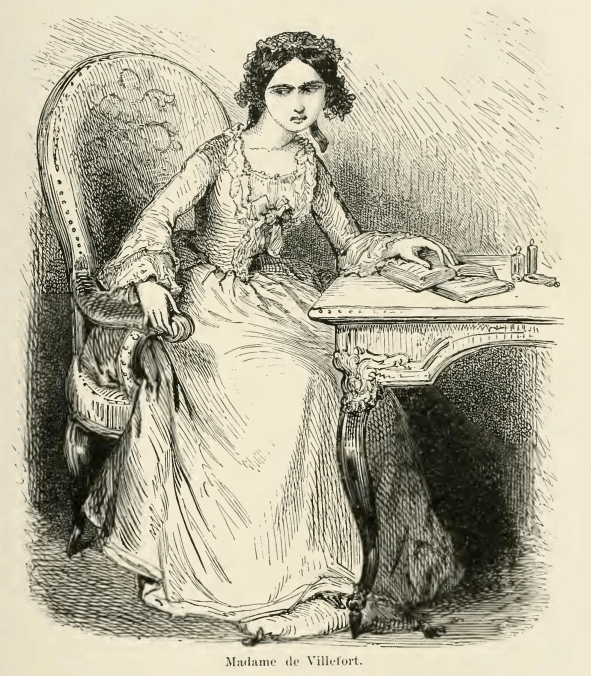
\includegraphics[width=\textwidth]{30023m.jpg}
\end{figure}

M. de Villefort was not only a magistrate, he was almost a diplomatist.
His relations with the former court, of which he always spoke with
dignity and respect, made him respected by the new one, and he knew so
many things, that not only was he always carefully considered, but
sometimes consulted. Perhaps this would not have been so had it been
possible to get rid of M. de Villefort; but, like the feudal barons who
rebelled against their sovereign, he dwelt in an impregnable fortress.
This fortress was his post as king’s attorney, all the advantages of
which he exploited with marvellous skill, and which he would not have
resigned but to be made deputy, and thus to replace neutrality by
opposition.

Ordinarily M. de Villefort made and returned very few visits. His wife
visited for him, and this was the received thing in the world, where
the weighty and multifarious occupations of the magistrate were
accepted as an excuse for what was really only calculated pride, a
manifestation of professed superiority—in fact, the application of the
axiom, \textit{Pretend to think well of yourself, and the world will think
well of you}, an axiom a hundred times more useful in society nowadays
than that of the Greeks, “Know thyself,” a knowledge for which, in our
days, we have substituted the less difficult and more advantageous
science of \textit{knowing others}.

To his friends M. de Villefort was a powerful protector; to his
enemies, he was a silent, but bitter opponent; for those who were
neither the one nor the other, he was a statue of the law-made man. He
had a haughty bearing, a look either steady and impenetrable or
insolently piercing and inquisitorial. Four successive revolutions had
built and cemented the pedestal upon which his fortune was based.

M. de Villefort had the reputation of being the least curious and the
least wearisome man in France. He gave a ball every year, at which he
appeared for a quarter of an hour only,—that is to say, five-and-forty
minutes less than the king is visible at his balls. He was never seen
at the theatres, at concerts, or in any place of public resort.
Occasionally, but seldom, he played at whist, and then care was taken
to select partners worthy of him—sometimes they were ambassadors,
sometimes archbishops, or sometimes a prince, or a president, or some
dowager duchess.

Such was the man whose carriage had just now stopped before the Count
of Monte Cristo’s door. The valet de chambre announced M. de Villefort
at the moment when the count, leaning over a large table, was tracing
on a map the route from St. Petersburg to China.

The procureur entered with the same grave and measured step he would
have employed in entering a court of justice. He was the same man, or
rather the development of the same man, whom we have heretofore seen as
assistant attorney at Marseilles. Nature, according to her way, had
made no deviation in the path he had marked out for himself. From being
slender he had now become meagre; once pale, he was now yellow; his
deep-set eyes were hollow, and the gold spectacles shielding his eyes
seemed to be an integral portion of his face. He dressed entirely in
black, with the exception of his white tie, and his funeral appearance
was only mitigated by the slight line of red ribbon which passed almost
imperceptibly through his button-hole, and appeared like a streak of
blood traced with a delicate brush.

Although master of himself, Monte Cristo, scrutinized with
irrepressible curiosity the magistrate whose salute he returned, and
who, distrustful by habit, and especially incredulous as to social
prodigies, was much more despised to look upon “the noble stranger,” as
Monte Cristo was already called, as an adventurer in search of new
fields, or an escaped criminal, rather than as a prince of the Holy
See, or a sultan of the \textit{Thousand and One Nights}.

“Sir,” said Villefort, in the squeaky tone assumed by magistrates in
their oratorical periods, and of which they cannot, or will not, divest
themselves in society, “sir, the signal service which you yesterday
rendered to my wife and son has made it a duty for me to offer you my
thanks. I have come, therefore, to discharge this duty, and to express
to you my overwhelming gratitude.”

And as he said this, the “eye severe” of the magistrate had lost
nothing of its habitual arrogance. He spoke in a voice of the
procureur-general, with the rigid inflexibility of neck and shoulders
which caused his flatterers to say (as we have before observed) that he
was the living statue of the law.

“Monsieur,” replied the count, with a chilling air, “I am very happy to
have been the means of preserving a son to his mother, for they say
that the sentiment of maternity is the most holy of all; and the good
fortune which occurred to me, monsieur, might have enabled you to
dispense with a duty which, in its discharge, confers an undoubtedly
great honor; for I am aware that M. de Villefort is not usually lavish
of the favor which he now bestows on me,—a favor which, however
estimable, is unequal to the satisfaction which I have in my own
consciousness.”

Villefort, astonished at this reply, which he by no means expected,
started like a soldier who feels the blow levelled at him over the
armor he wears, and a curl of his disdainful lip indicated that from
that moment he noted in the tablets of his brain that the Count of
Monte Cristo was by no means a highly bred gentleman.

He glanced around, in order to seize on something on which the
conversation might turn, and seemed to fall easily on a topic. He saw
the map which Monte Cristo had been examining when he entered, and
said:

“You seem geographically engaged, sir? It is a rich study for you, who,
as I learn, have seen as many lands as are delineated on this map.”

“Yes, sir,” replied the count; “I have sought to make of the human
race, taken in the mass, what you practice every day on individuals—a
physiological study. I have believed it was much easier to descend from
the whole to a part than to ascend from a part to the whole. It is an
algebraic axiom, which makes us proceed from a known to an unknown
quantity, and not from an unknown to a known; but sit down, sir, I beg
of you.”

Monte Cristo pointed to a chair, which the procureur was obliged to
take the trouble to move forwards himself, while the count merely fell
back into his own, on which he had been kneeling when M. Villefort
entered. Thus the count was halfway turned towards his visitor, having
his back towards the window, his elbow resting on the geographical
chart which furnished the theme of conversation for the moment,—a
conversation which assumed, as in the case of the interviews with
Danglars and Morcerf, a turn analogous to the persons, if not to the
situation.

“Ah, you philosophize,” replied Villefort, after a moment’s silence,
during which, like a wrestler who encounters a powerful opponent, he
took breath; “well, sir, really, if, like you, I had nothing else to
do, I should seek a more amusing occupation.”

“Why, in truth, sir,” was Monte Cristo’s reply, “man is but an ugly
caterpillar for him who studies him through a solar microscope; but you
said, I think, that I had nothing else to do. Now, really, let me ask,
sir, have you?—do you believe you have anything to do? or to speak in
plain terms, do you really think that what you do deserves being called
anything?”

Villefort’s astonishment redoubled at this second thrust so forcibly
made by his strange adversary. It was a long time since the magistrate
had heard a paradox so strong, or rather, to say the truth more
exactly, it was the first time he had ever heard of it. The procureur
exerted himself to reply.

“Sir,” he responded, “you are a stranger, and I believe you say
yourself that a portion of your life has been spent in Oriental
countries, so you are not aware how human justice, so expeditious in
barbarous countries, takes with us a prudent and well-studied course.”

“Oh, yes—yes, I do, sir; it is the \textit{pede claudo} of the ancients. I
know all that, for it is with the justice of all countries especially
that I have occupied myself—it is with the criminal procedure of all
nations that I have compared natural justice, and I must say, sir, that
it is the law of primitive nations, that is, the law of retaliation,
that I have most frequently found to be according to the law of God.”

“If this law were adopted, sir,” said the procureur, “it would greatly
simplify our legal codes, and in that case the magistrates would not
(as you just observed) have much to do.”

“It may, perhaps, come to this in time,” observed Monte Cristo; “you
know that human inventions march from the complex to the simple, and
simplicity is always perfection.”

“In the meanwhile,” continued the magistrate, “our codes are in full
force, with all their contradictory enactments derived from Gallic
customs, Roman laws, and Frank usages; the knowledge of all which, you
will agree, is not to be acquired without extended labor; it needs
tedious study to acquire this knowledge, and, when acquired, a strong
power of brain to retain it.”

“I agree with you entirely, sir; but all that even you know with
respect to the French code, I know, not only in reference to that code,
but as regards the codes of all nations. The English, Turkish,
Japanese, Hindu laws, are as familiar to me as the French laws, and
thus I was right, when I said to you, that relatively (you know that
everything is relative, sir)—that relatively to what I have done, you
have very little to do; but that relatively to all I have learned, you
have yet a great deal to learn.”

“But with what motive have you learned all this?” inquired Villefort,
in astonishment.

Monte Cristo smiled.

“Really, sir,” he observed, “I see that in spite of the reputation
which you have acquired as a superior man, you look at everything from
the material and vulgar view of society, beginning with man, and ending
with man—that is to say, in the most restricted, most narrow view which
it is possible for human understanding to embrace.”

“Pray, sir, explain yourself,” said Villefort, more and more
astonished, “I really do—not—understand you—perfectly.”

“I say, sir, that with the eyes fixed on the social organization of
nations, you see only the springs of the machine, and lose sight of the
sublime workman who makes them act; I say that you do not recognize
before you and around you any but those office-holders whose
commissions have been signed by a minister or king; and that the men
whom God has put above those office-holders, ministers, and kings, by
giving them a mission to follow out, instead of a post to fill—I say
that they escape your narrow, limited field of observation. It is thus
that human weakness fails, from its debilitated and imperfect organs.
Tobias took the angel who restored him to light for an ordinary young
man. The nations took Attila, who was doomed to destroy them, for a
conqueror similar to other conquerors, and it was necessary for both to
reveal their missions, that they might be known and acknowledged; one
was compelled to say, ‘I am the angel of the Lord’; and the other, ‘I
am the hammer of God,’ in order that the divine essence in both might
be revealed.”

“Then,” said Villefort, more and more amazed, and really supposing he
was speaking to a mystic or a madman, “you consider yourself as one of
those extraordinary beings whom you have mentioned?”

“And why not?” said Monte Cristo coldly.

“Your pardon, sir,” replied Villefort, quite astounded, “but you will
excuse me if, when I presented myself to you, I was unaware that I
should meet with a person whose knowledge and understanding so far
surpass the usual knowledge and understanding of men. It is not usual
with us corrupted wretches of civilization to find gentlemen like
yourself, possessors, as you are, of immense fortune—at least, so it is
said—and I beg you to observe that I do not inquire, I merely
repeat;—it is not usual, I say, for such privileged and wealthy beings
to waste their time in speculations on the state of society, in
philosophical reveries, intended at best to console those whom fate has
disinherited from the goods of this world.”

“Really, sir,” retorted the count, “have you attained the eminent
situation in which you are, without having admitted, or even without
having met with exceptions? and do you never use your eyes, which must
have acquired so much \textit{finesse} and certainty, to divine, at a glance,
the kind of man by whom you are confronted? Should not a magistrate be
not merely the best administrator of the law, but the most crafty
expounder of the chicanery of his profession, a steel probe to search
hearts, a touchstone to try the gold which in each soul is mingled with
more or less of alloy?”

“Sir,” said Villefort, “upon my word, you overcome me. I really never
heard a person speak as you do.”

“Because you remain eternally encircled in a round of general
conditions, and have never dared to raise your wings into those upper
spheres which God has peopled with invisible or exceptional beings.”

“And you allow then, sir, that spheres exist, and that these marked and
invisible beings mingle amongst us?”

“Why should they not? Can you see the air you breathe, and yet without
which you could not for a moment exist?”

“Then we do not see those beings to whom you allude?”

“Yes, we do; you see them whenever God pleases to allow them to assume
a material form. You touch them, come in contact with them, speak to
them, and they reply to you.”

“Ah,” said Villefort, smiling, “I confess I should like to be warned
when one of these beings is in contact with me.”

“You have been served as you desire, monsieur, for you were warned just
now, and I now again warn you.”

“Then you yourself are one of these marked beings?”

“Yes, monsieur, I believe so; for until now, no man has found himself
in a position similar to mine. The dominions of kings are limited
either by mountains or rivers, or a change of manners, or an alteration
of language. My kingdom is bounded only by the world, for I am not an
Italian, or a Frenchman, or a Hindu, or an American, or a Spaniard—I am
a cosmopolite. No country can say it saw my birth. God alone knows what
country will see me die. I adopt all customs, speak all languages. You
believe me to be a Frenchman, for I speak French with the same facility
and purity as yourself. Well, Ali, my Nubian, believes me to be an
Arab; Bertuccio, my steward, takes me for a Roman; Haydée, my slave,
thinks me a Greek. You may, therefore, comprehend, that being of no
country, asking no protection from any government, acknowledging no man
as my brother, not one of the scruples that arrest the powerful, or the
obstacles which paralyze the weak, paralyzes or arrests me. I have only
two adversaries—I will not say two conquerors, for with perseverance I
subdue even them,—they are time and distance. There is a third, and the
most terrible—that is my condition as a mortal being. This alone can
stop me in my onward career, before I have attained the goal at which I
aim, for all the rest I have reduced to mathematical terms. What men
call the chances of fate—namely, ruin, change, circumstances—I have
fully anticipated, and if any of these should overtake me, yet it will
not overwhelm me. Unless I die, I shall always be what I am, and
therefore it is that I utter the things you have never heard, even from
the mouths of kings—for kings have need, and other persons have fear of
you. For who is there who does not say to himself, in a society as
incongruously organized as ours, ‘Perhaps some day I shall have to do
with the king’s attorney’?”

“But can you not say that, sir? The moment you become an inhabitant of
France, you are naturally subjected to the French law.”

“I know it sir,” replied Monte Cristo; “but when I visit a country I
begin to study, by all the means which are available, the men from whom
I may have anything to hope or to fear, till I know them as well as,
perhaps better than, they know themselves. It follows from this, that
the king’s attorney, be he who he may, with whom I should have to deal,
would assuredly be more embarrassed than I should.”

“That is to say,” replied Villefort with hesitation, “that human nature
being weak, every man, according to your creed, has committed faults.”

“Faults or crimes,” responded Monte Cristo with a negligent air.

“And that you alone, amongst the men whom you do not recognize as your
brothers—for you have said so,” observed Villefort in a tone that
faltered somewhat—“you alone are perfect.”

“No, not perfect,” was the count’s reply; “only impenetrable, that’s
all. But let us leave off this strain, sir, if the tone of it is
displeasing to you; I am no more disturbed by your justice than are you
by my second-sight.”

“No, no,—by no means,” said Villefort, who was afraid of seeming to
abandon his ground. “No; by your brilliant and almost sublime
conversation you have elevated me above the ordinary level; we no
longer talk, we rise to dissertation. But you know how the theologians
in their collegiate chairs, and philosophers in their controversies,
occasionally say cruel truths; let us suppose for the moment that we
are theologizing in a social way, or even philosophically, and I will
say to you, rude as it may seem, ‘My brother, you sacrifice greatly to
pride; you may be above others, but above you there is God.’”

\begin{figure}[ht]
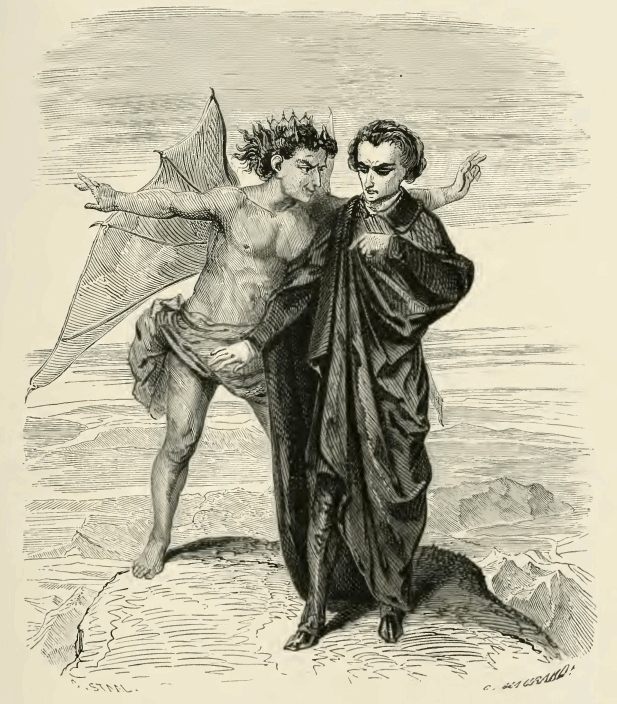
\includegraphics[width=\textwidth]{30029m.jpg}
\end{figure}

“Above us all, sir,” was Monte Cristo’s response, in a tone and with an
emphasis so deep that Villefort involuntarily shuddered. “I have my
pride for men—serpents always ready to threaten everyone who would pass
without crushing them under foot. But I lay aside that pride before
God, who has taken me from nothing to make me what I am.”

“Then, count, I admire you,” said Villefort, who, for the first time in
this strange conversation, used the aristocratic form to the unknown
personage, whom, until now, he had only called monsieur. “Yes, and I
say to you, if you are really strong, really superior, really pious, or
impenetrable, which you were right in saying amounts to the same
thing—then be proud, sir, for that is the characteristic of
predominance. Yet you have unquestionably some ambition.”

“I have, sir.”

“And what may it be?”

“I too, as happens to every man once in his life, have been taken by
Satan into the highest mountain in the earth, and when there he showed
me all the kingdoms of the world, and as he said before, so said he to
me, ‘Child of earth, what wouldst thou have to make thee adore me?’ I
reflected long, for a gnawing ambition had long preyed upon me, and
then I replied, ‘Listen,—I have always heard of Providence, and yet I
have never seen him, or anything that resembles him, or which can make
me believe that he exists. I wish to be Providence myself, for I feel
that the most beautiful, noblest, most sublime thing in the world, is
to recompense and punish.’ Satan bowed his head, and groaned. ‘You
mistake,’ he said, ‘Providence does exist, only you have never seen
him, because the child of God is as invisible as the parent. You have
seen nothing that resembles him, because he works by secret springs,
and moves by hidden ways. All I can do for you is to make you one of
the agents of that Providence.’ The bargain was concluded. I may
sacrifice my soul, but what matters it?” added Monte Cristo. “If the
thing were to do again, I would again do it.”

Villefort looked at Monte Cristo with extreme amazement.

“Count,” he inquired, “have you any relations?”

“No, sir, I am alone in the world.”

“So much the worse.”

“Why?” asked Monte Cristo.

“Because then you might witness a spectacle calculated to break down
your pride. You say you fear nothing but death?”

“I did not say that I feared it; I only said that death alone could
check the execution of my plans.”

“And old age?”

“My end will be achieved before I grow old.”

“And madness?”

“I have been nearly mad; and you know the axiom,—\textit{non bis in idem}. It
is an axiom of criminal law, and, consequently, you understand its full
application.”

\begin{figure}[ht]
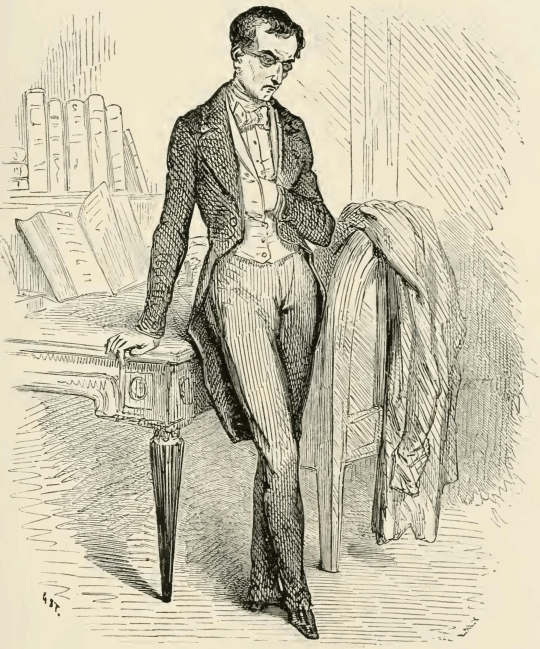
\includegraphics[width=\textwidth]{30031m.jpg}
\end{figure}

“Sir,” continued Villefort, “there is something to fear besides death,
old age, and madness. For instance, there is apoplexy—that
lightning-stroke which strikes but does not destroy you, and yet which
brings everything to an end. You are still yourself as now, and yet you
are yourself no longer; you who, like Ariel, verge on the angelic, are
but an inert mass, which, like Caliban, verges on the brutal; and this
is called in human tongues, as I tell you, neither more nor less than
apoplexy. Come, if so you will, count, and continue this conversation
at my house, any day you may be willing to see an adversary capable of
understanding and anxious to refute you, and I will show you my father,
M. Noirtier de Villefort, one of the most fiery Jacobins of the French
Revolution; that is to say, he had the most remarkable audacity,
seconded by a most powerful organization—a man who has not, perhaps,
like yourself seen all the kingdoms of the earth, but who has helped to
overturn one of the greatest; in fact, a man who believed himself, like
you, one of the envoys, not of God, but of a supreme being; not of
Providence, but of fate. Well, sir, the rupture of a blood-vessel on
the lobe of the brain has destroyed all this, not in a day, not in an
hour, but in a second. M. Noirtier, who, on the previous night, was the
old Jacobin, the old senator, the old Carbonaro, laughing at the
guillotine, the cannon, and the dagger—M. Noirtier, playing with
revolutions—M. Noirtier, for whom France was a vast chess-board, from
which pawns, rooks, knights, and queens were to disappear, so that the
king was checkmated—M. Noirtier, the redoubtable, was the next morning
\textit{poor M. Noirtier}, the helpless old man, at the tender mercies of the
weakest creature in the household, that is, his grandchild, Valentine;
a dumb and frozen carcass, in fact, living painlessly on, that time may
be given for his frame to decompose without his consciousness of its
decay.”

“Alas, sir,” said Monte Cristo “this spectacle is neither strange to my
eye nor my thought. I am something of a physician, and have, like my
fellows, sought more than once for the soul in living and in dead
matter; yet, like Providence, it has remained invisible to my eyes,
although present to my heart. A hundred writers since Socrates, Seneca,
St. Augustine, and Gall, have made, in verse and prose, the comparison
you have made, and yet I can well understand that a father’s sufferings
may effect great changes in the mind of a son. I will call on you, sir,
since you bid me contemplate, for the advantage of my pride, this
terrible spectacle, which must have been so great a source of sorrow to
your family.”

“It would have been so unquestionably, had not God given me so large a
compensation. In contrast with the old man, who is dragging his way to
the tomb, are two children just entering into life—Valentine, the
daughter by my first wife—Mademoiselle Renée de Saint-Méran—and Edward,
the boy whose life you have this day saved.”

“And what is your deduction from this compensation, sir?” inquired
Monte Cristo.

“My deduction is,” replied Villefort, “that my father, led away by his
passions, has committed some fault unknown to human justice, but marked
by the justice of God. That God, desirous in his mercy to punish but
one person, has visited this justice on him alone.”

Monte Cristo with a smile on his lips, uttered in the depths of his
soul a groan which would have made Villefort fly had he but heard it.

“Adieu, sir,” said the magistrate, who had risen from his seat; “I
leave you, bearing a remembrance of you—a remembrance of esteem, which
I hope will not be disagreeable to you when you know me better; for I
am not a man to bore my friends, as you will learn. Besides, you have
made an eternal friend of Madame de Villefort.”

The count bowed, and contented himself with seeing Villefort to the
door of his cabinet, the procureur being escorted to his carriage by
two footmen, who, on a signal from their master, followed him with
every mark of attention. When he had gone, Monte Cristo breathed a
profound sigh, and said:

“Enough of this poison, let me now seek the antidote.”

Then sounding his bell, he said to Ali, who entered:

“I am going to madame’s chamber—have the carriage ready at one
o’clock.”
